\documentclass[french]{article}

% Packages
\usepackage[utf8]{inputenc}
\usepackage[T1]{fontenc}
\usepackage{babel}
\usepackage{caption}
\usepackage{graphicx}
\usepackage{hyperref}
\usepackage{authblk}

% Article
\author{Matthieu Giraud%
\thanks{Adresse e-mail : \texttt{matthieu.giraud@uca.fr}}}

\date{}

\title{Effectuer des recherches sur des données chiffrées}
\affil{\textsc{limos}, Université Clermont Auvergne}

\begin{document}

\maketitle

Le développement d'Internet ces dernières années offre à l'utilisateur
de nombreux services numériques. Parmi eux, nous avons aujourd'hui :
la recherche d'information (Wikipédia), la musique en streaming
(Deezer, Spotify), la vidéo à la demande (YouTube, Netflix), les
réseaux sociaux (Facebook, Twitter) ou encore la sauvegarde de données
en ligne (Dropbox, Google Drive). C'est sur ce dernier service, la
sauvegarde de données en ligne, également désigné par le terme
d'externalisation de données dans le Cloud, que nous nous focalisons
dans cet article.

Le stockage de données en ligne a de nombreux avantages pour
l'utilisateur.  En effet, il permet à celui-ci d'avoir une sauvegarde
de ses données même si son matériel informatique tombe en
panne. D'autre part, si l'utilisateur est amené à se déplacer
régulièrement, le stockage de ses données en ligne lui permettra d'y
avoir accès facilement quelque soit l'endroit où il se trouve à
condition d'avoir une connexion à Internet.

Bien entendu ces avantages conduisent à des questions de
confidentialité des données et au respect de la vie privée. Supposons
que les données que souhaitent sauvegarder l'utilisateur soient des
données dites sensibles ou à caractère personnel. Il peut s'agir par
exemple de ses relevés bancaires, de ses photos personnelles ou de ses
résultats médicaux. Dans ce cas, l'utilisateur devra faire confiance
au service de stockage en ligne à qui il confie ses données. Cette
confiance repose sur deux points. Le premier concerne la sécurité de
l'infrastructure informatique du service Cloud lui-même
(Figure~\ref{fig:threat1}). Si le serveur sauvegardant les données du
client possède des failles informatiques (non mise à jour du système
d'exploitation, absence d'anti-virus, etc.), une personne malveillante
pouvant exploiter ces failles serait alors en mesure de récupérer les
données de l'utilisateur ou encore de les détruire. Le second point
concerne la position du service Cloud par rapport aux données qu'il
sauvegarde ; rien n'empêche celui-ci de regarder par curiosité ou par
intérêts économiques les données que son client héberge sur ses
propres serveurs (Figure~\ref{fig:threat2}).

\begin{center}
  \begin{minipage}[t]{.49\linewidth}
    \centering
    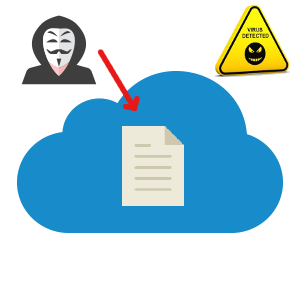
\includegraphics[scale=.4]{images/threat1.png}
    \captionof{figure}{Sécurité du Cloud.}
    \label{fig:threat1}
  \end{minipage}
  \hfill
  \begin{minipage}[t]{.49\linewidth}
    \centering
    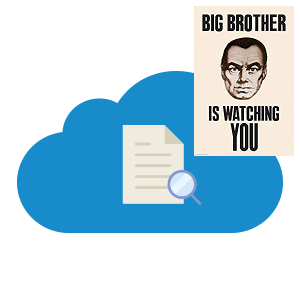
\includegraphics[scale=.4]{images/threat2.png}
    \captionof{figure}{Curiosité du Cloud.}
    \label{fig:threat2}
  \end{minipage}
\end{center}

Afin de protéger ces données externalisées face à de telles menaces,
une première solution est d'utiliser un schéma de chiffrement
symétrique. La sécurité d'un chiffrement symétrique repose sur la
connaissance d'un secret. Ce secret correspond à la clef secrète
permettant à l'utilisateur de chiffrer, puis de déchiffrer ses
données.  Ainsi, si l'utilisateur exporte ses données sur un service
de stockage en ligne une fois les avoir chiffrées à l'aide d'un schéma
de chiffrement et de sa clef secrète, il aura alors la garantie que
personne d'autre que lui ne pourra exploiter ses données puisque
lui-seul possède la clef secrète permettant le
déchiffrement. Néanmoins, le fait de chiffrer les données
externalisées enlève à l'utilisateur la possibilité d'exploiter
celles-ci directement en ligne. En effet, traiter ses documents
directement en ligne revient à dire que le serveur possède la clef de
déchiffrement de l'utilisateur. Ainsi, il est impossible pour
l'utilisateur de regarder ses photos, de modifier un document texte,
de faire des recherches par mots-clefs sur les documents,
etc. directement en ligne. L'utilisateur devra donc tout d'abord
télécharger toutes ses données depuis le service Cloud sur son
ordinateur, les déchiffrer, faire la manipulation souhaitée puis les
chiffrer de nouveau avant de les exporter une nouvelle fois sur le
service de stockage en ligne. Cette méthode, bien que sécurisée contre
les menaces citées précédemment n'est pas pratique pour l'utilisateur.

Une solution consiste à utiliser un schéma de chiffrement dit
homomorphique. Un tel chiffrement permet d'effectuer les mêmes
opérations sur des données chiffrées que sur des données claires. Par
exemple, si l'utilisateur a créé deux chiffrés : $c_1$ correspondant
au message $m_1 = 2000$ et $c_2$ correspondant au message $m_2 = 18$,
alors l'addition des deux chiffrés $c_1 + c_2$ donnera le message
$2018$ après déchiffrement. Ainsi, grâce à un tel chiffrement,
l'utilisateur n'a plus besoin de télécharger ses données chiffrées et
de les déchiffrer pour appliquer l'opération souhaitée. Il peut
directement manipuler ses données chiffrées à distance et y appliquer
les modifications qu'il souhaite. Hélas, ces chiffrements demandent un
temps de calcul trop important. Ainsi, nous avons d'un côté une
solution sécurisée et efficace mais sans fonctionnalités et d'un autre
côté une solution sécurisée avec fonctionnalités mais inefficace.

Néanmoins, il existe un compromis entre sécurité, performance et
fonctionnalité pour la fonctionnalité de recherche par mots-clefs sur
des données chiffrées ; ce sont les schémas de recherche sur données
chiffrées, appelés en anglais \emph{Searchable Encryptions}.

La fonctionnalité de recherche par mots-clefs sur des données
chiffrées permet à l'utilisateur de récupérer, parmi une liste de
documents chiffrés, ceux contenant les mots-clefs recherchés.

Le premier schéma de recherche sur données chiffrées a été proposé par
Song, Wagner et Perrig en 2000~\cite{SongWP00} et ne proposait que la
recherche via un seul mot-clef. Depuis, de nombreux autres schémas ont
été proposés apportant des améliorations. Certains d'entre eux
permettent d'ajouter de nouveaux documents~\cite{KamaraPR12} tout en
permettant d'effectuer des recherches, et d'autres schémas permettent
à l'utilisateur d'effectuer des recherches plus
complexes~\cite{CashJJKRS13}, dites booléennes, comme vouloir que deux
mots-clefs soient présents simultanément dans les documents retournés
sans que ceux-là n'en contiennent un troisième.

Certains schémas de recherche par mots-clefs sur des données chiffrées
permettent d'effectuer des recherche grâce à la structure même des
documents chiffrés, d'autres sont basés sur une structure appelée
index inversée. Un index inversé est une structure permettant de
ranger un ensemble de documents en fonction des mots-clefs qui les
composent. Supposons par exemple que nous avons deux documents nommés
$d_1$ et $d_2$, et définis par :

\begin{itemize}
\item $d_1$ : ``La sécurité informatique est importante''
\item $d_2$ : ``L'informatique est omniprésente''
\end{itemize}

Pour construire l'index inversé associé à ces deux documents, il
suffit de prendre chacun des mots-clefs composant ces deux documents
et lui associer le nom des documents qui le contient. Avec les deux
documents précédents $d_1$ et $d_2$, nous obtenons l'index inversé
présenté dans la Figure~\ref{fig:indexinv}.

\begin{figure}[h]
  \centering
  \begin{tabular}{|c|c|}
    \hline
    Mots-clefs & Documents associés \\
    \hline
    sécurité & $d_1$ \\
    \hline
    informatique & $d_1$ $d_2$ \\
    \hline
    importante & $d_1$ \\
    \hline
    omniprésente & $d_2$ \\
    \hline
  \end{tabular}
  \caption{Index inversé.}
  \label{fig:indexinv}
\end{figure}

Ainsi, lorsque l'utilisateur recherche les documents contenant le
mot-clef \textit{informatique}, celui-ci grâce à l'index inversé,
saura que les deux documents $d_1$ et $d_2$ contiennent ce mot-clef.

Nous allons voir maintenant comment utiliser la structure de l'index
inversé pour qu'un utilisateur puisse effectuer une recherche avec un
mot-clef de façon sécurisée. Nous souhaitons que l'utilisateur puisse
effectuer une recherche sur des documents chiffrées sans que le
service cloud puisse connaître le sens du mot-clef fourni par
l'utilisateur.

Supposons tout d'abord qu'un utilisateur possède les deux documents
$d_1$ et $d_2$ cités précédemment et qu'il souhaite les externaliser
sur un service de stockage en ligne. La première étape pour
l'utilisateur est de créer ce que nous appelons l'index inversé
chiffré associé à cet ensemble documentaire. Pour cela, il choisit
d'abord deux clefs secrètes que nous nommerons $k_1$ et $k_2$. À
l'aide d'une fonction dite pseudo-aléatoire~\cite{GGM86} associée à la
clef secrète $k_1$, l'utilisateur protège les mots-clefs de l'index
inversé (présenté à la Figure~\ref{fig:indexinv}) en remplaçant chacun
d'eux par la valeur donnée par la fonction aléatoire. Si le mot-clef
considéré est \textit{informatique} alors la valeur donnée par la
fonction pseudo-aléatoire associée à la clef $k_1$ sera notée
$\{\mathit{informatique}\}_{k_1}$. Il est important de comprendre que
cette valeur est incompréhensible pour le service cloud, en d'autres
termes le mot-clef \textit{informatique} est remplacée par une valeur
d'apparence aléatoire mais dépendant de la clef secrète $k_1$.

Ensuite, l'utilisateur utilise sa deuxième clef secrète $k_2$ pour
chiffrer ses documents, ici : $d_1$ et $d_2$. Nous indiquons les
chiffrés de ces deux documents à l'aide de la clef secrète $k_2$ par
les notations suivantes : $d_1^*$ et $d_2^*$. Ainsi, l'index inversé
ne fait plus le lien entre les mots-clefs et les documents originaux
de l'utilisateur mais fait le lien entre les mots-clefs protégés
(i.e. les valeurs pseudo-aléatoires associées aux mots-clefs) et les
documents chiffrés de l'utilisateur. Ces documents chiffrés sont
calculés par l'utilisateur en utilisant par exemple l'algorithme de
chiffrement
\href{https://fr.wikipedia.org/wiki/Advanced_Encryption_Standard}{AES}
avec la clef secrète $k_2$. Nous illustrons l'index inversé chiffré
associés aux documents $d_1$ et $d_2$ dans la
figure~\ref{fig:encindexinv}.

\begin{figure}[h]
  \centering
  \begin{tabular}{|c|c|}
    \hline
    Mots-clefs & Documents associés \\
    \hline
    $\{\textrm{s\'ecurit\'e}\}_{k_1}$ & $d_1^*$ \\
    \hline
    $\{\textrm{informatique}\}_{k_1}$ & $d_1^*$ $d_2^*$ \\
    \hline
    $\{\textrm{importante}\}_{k_1}$ & $d_1^*$ \\
    \hline
    $\{\textrm{omnipr\'esente}\}_{k_1}$ & $d_2^*$ \\
    \hline
  \end{tabular}
  \caption{Index inversé chiffré.}
  \label{fig:encindexinv}
\end{figure}

Une fois cet index inversé chiffré et ces documents chiffrés générés
par l'utilisateur, celui-ci les exporte sur le service de stockage en
ligne (l'utilisateur n'est ensuite pas obligé de garder les documents
originaux sur son ordinateur). Grâce au chiffrement des documents,
ceux-là sont protégés. De plus, l'index inversé chiffré permet à
l'utilisateur d'effectuer des recherches par mots-clefs sur ses
documents chiffrés. En effet, connaissant la clef secrète $k_1$,
l'utilisateur souhaitant récupérer les documents contenant le mot-clef
``informatique'' calcule alors la valeur pseudo-alétoire associé à ce
mot-clef, i.e. $\{\textrm{informatique}\}_{k_1}$. L'utilisateur envoie
ensuite cette valeur calculée au service cloud. Grâce à l'index
inversée chiffrée (Figure~\ref{fig:encindexinv}), le service cloud
sait que les documents chiffrés $d_1^*$ et $d_2^*$ sont associés à
cette valeur pseudo-aléatoire et les envoie donc à
l'utilisateur. L'utilisateur connaissant sa deuxième clef secrète
$k_2$ peut ainsi déchiffrer les deux documents chiffrés reçus
correspondant à sa recherche.

Ainsi, nous venons de voir que les schémas de recherches sur données
chiffrées permettent à un utilisateur de sauvegarder ses données
chiffrées dans le cloud tout en lui permettant d'effectuer des
recherches par mots-clefs. Aujourd'hui de nombreuses solutions
commerciales telles que \emph{CipherCloud}, \emph{Skyhigh Networks} ou
encore \emph{bitglass} proposent un tel service aux
internautes. Toutefois des recherches récentes~\cite{GiraudABL17} ont
mis en évidence certaines menaces sur les schémas de recherches sur
données chiffrées basés sur les index inversés. En effet, si le
serveur hébergeant ces documents chiffrés connaît un petit échantillon
de documents qu'il héberge, il sera alors en mesure d'obtenir d'autres
informations sur les autres documents. La recherche actuelle se porte
sur des contre-mesures et de nouveaux modèles de schémas de recherche,
afin d'éviter de telles fuites d'information pour garantir la sécurité
des données personnelles hébergées dans le cloud.

\bibliography{references}{}
\bibliographystyle{plain}

\end{document}
